\documentclass[11pt,a4paper]{article}

\usepackage[brazil]{babel}
\usepackage[T1]{fontenc}
\usepackage{lmodern}
\usepackage{microtype}
\usepackage[margin=2.2cm]{geometry}
\usepackage{amsmath}
\usepackage{booktabs}
\usepackage{tabularx}
\usepackage{enumitem}
\usepackage{graphicx}
\usepackage{float}
\usepackage{caption}
\usepackage{xcolor}
\usepackage[hidelinks]{hyperref}

\setlist{nosep, leftmargin=*}
\setlength{\parskip}{0.4em}
\setlength{\parindent}{0pt}
\captionsetup{font=small, labelfont=bf}
\graphicspath{{figuras/}}

% Trechos que ainda dependem dos experimentos de custo.
\newcommand{\pendente}[1]{\textcolor{red!70!black}{\textbf{[pendente:} #1\textbf{]}}}

\title{\textbf{A* no Lago Congelado: variações de cenário e de custo}\\[0.3em]
  \large Relatório de experimentos}
\author{Luisa Ferreira \quad Caio Trindade\\
  \small Inteligência Artificial para Jogos I --- Aula 27, pathfinding}
\date{Novembro de 2026}

\begin{document}
\maketitle

\textbf{Código:} o notebook adaptado, com a implementação, os experimentos e todas as saídas, é o arquivo
\texttt{frozenlake\_astar.ipynb}. A busca fica no módulo \texttt{astar.py}, os geradores de mapa em
\texttt{cenarios.py} e as camadas de custo em \texttt{custos.py}. Tudo está disponível em:\\
\url{https://github.com/ctrindadedev/game-ai-lab/tree/master/FrozenLake}

O ponto de partida é o notebook da disciplina (\texttt{Pratica\_2\_Completa.ipynb}, link do slide 36), que roda o A*
com distância Manhattan e custo 1 por passo num mapa 8x8. Em aula a busca foi mostrada só nesse cenário simples. Este
trabalho explora o A* em dois eixos: \textbf{o cenário} (tamanho do grid, posições do início e do objetivo, buracos) e
\textbf{o custo da rota}, com o Uber como inspiração (terreno, segurança e tráfego).

O A* expande sempre o nó da fronteira com menor
\[
f(n) = g(n) + h(n),
\]
em que $g(n)$ é o custo real do início até $n$ e $h(n)$ é a estimativa de $n$ até o objetivo. Se $h$ nunca superestima
o custo real (heurística \emph{admissível}), o primeiro caminho que chega ao objetivo é ótimo. A pergunta do trabalho
é como o cenário e a função de custo afetam duas coisas: a qualidade do caminho e o esforço da busca.

\section{Ambientes}

\subsection*{FrozenLake-v1 (Lago Congelado), versão determinística}

\begin{itemize}
  \item \textbf{Estados:} a célula $(\text{linha}, \text{coluna})$ do grid, que no Gymnasium vira o índice
    $\text{linha} \times n + \text{coluna}$. Os mapas vão de 4x4 (16 estados) a 64x64 (4096 estados).
  \item \textbf{Ações:} 4, com a mesma numeração do Gymnasium (0 = esquerda, 1 = baixo, 2 = direita, 3 = cima).
  \item \textbf{Células:} \texttt{S} (início), \texttt{F} (gelo), \texttt{H} (buraco) e \texttt{G} (objetivo). Para a busca,
    os buracos são intransitáveis, porque cair num deles encerra o episódio.
  \item \textbf{Função de custo:} no eixo de cenário, cada passo custa 1, como em aula. No eixo de custo, cada passo
    custa de acordo com as camadas de terreno, segurança e tráfego da célula de destino:
    \[
      c(n \to n') = 1 + w_t\,(\text{terreno}(n') - 1) + w_s\,\text{insegurança}(n') + w_{tr}\,\text{tráfego}(n'),
    \]
    com terreno de 1 a 4, insegurança de 0 a 5 e tráfego de 0 a 3,5 no pico. Como os pesos e as penalidades são
    $\ge 0$, todo passo custa pelo menos 1. Nos mapas testados, o passo mais caro custa em média 6,0 no perfil mais
    rápido, 7,9 no equilibrado e 11,2 no mais seguro.
  \item \textbf{Reforço do Gymnasium:} $+1$ ao chegar ao \texttt{G} e $0$ nos demais passos. O A* não usa esse reforço
    para decidir; ele serve só para conferir, no ambiente real, que o caminho planejado chega ao objetivo.
  \item \textbf{Escorregadio:} desligado (\texttt{is\_slippery=False}). O A* planeja a sequência de ações inteira antes de
    agir, então precisa que cada ação leve exatamente à célula esperada.
\end{itemize}

\textbf{Dificuldades e desafios.} A distância Manhattan ignora os buracos. Quanto mais o mapa obriga a desviar, mais
ela subestima o custo real, e mais nós a busca precisa expandir. Em mapas grandes isso pesa: uma busca sem heurística
cresce com a área do mapa. Há ainda mapas sem caminho, em que a busca precisa terminar e informar isso. No eixo de custo,
o desafio passa a ser outro: com passos mais caros que 1, a Manhattan pura subestima demais, e uma heurística
``esperta'' pode passar a superestimar e quebrar a garantia de otimalidade.

\begin{figure}[H]
  \centering
  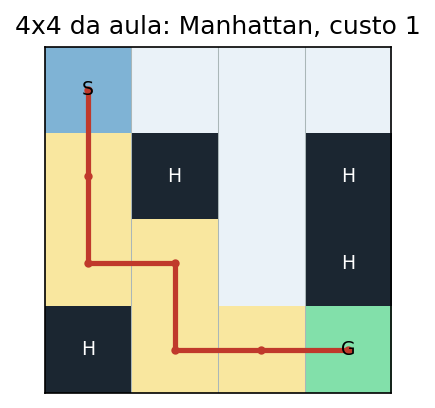
\includegraphics[width=0.36\linewidth]{mapa_aula.png}\hspace{1.5em}
  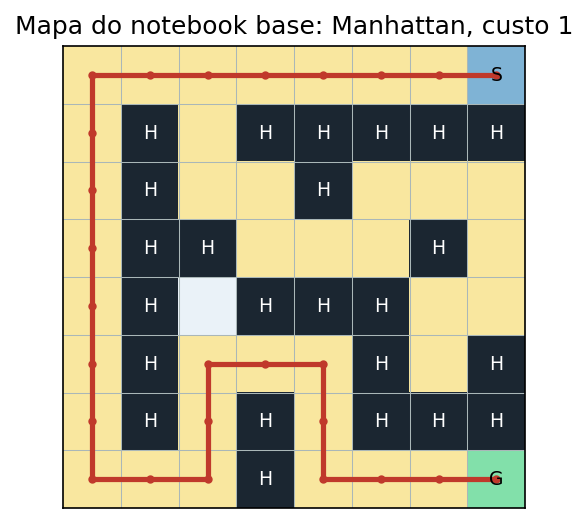
\includegraphics[width=0.36\linewidth]{mapa_base.png}
  \caption{À esquerda, o 4x4 da aula (g = 6, como nos slides 18 a 32). À direita, o mapa do notebook base: o G fica
    logo abaixo do S, mas a fileira de buracos obriga a dar a volta, e o A* expande 38 nós para um caminho de 25
    passos. Amarelo: células expandidas; vermelho: caminho.}
  \label{fig:base}
\end{figure}

\section{Metodologia experimental}

\subsection{Configuração dos experimentos}

\textbf{Implementação.} Cada nó guarda os 4 componentes do slide 35: \textbf{estado} (a célula), \textbf{nó pai},
\textbf{ação} que levou até ele e \textbf{custo do caminho} $g(n)$. A fronteira (abertos) é uma fila de prioridade
(\texttt{heapq}) ordenada por $f$. Os empates são desfeitos pelo menor $h$ e, depois, pela ordem de inserção. As células
expandidas vão para a lista de fechados, e o caminho é reconstruído seguindo os pais a partir do objetivo. A busca
recebe duas funções, \texttt{custo\_fn(origem, destino)} e \texttt{heuristica\_fn(célula, objetivo)}, e por isso os dois
eixos usam exatamente o mesmo A*.

\textbf{Parâmetros variados no eixo de cenário} (custo 1 por passo):
\begin{itemize}
  \item \textbf{tamanho do grid}: 4, 8, 16, 32 e 64, com 20 mapas do \texttt{generate\_random\_map} ($p = 0{,}8$) por tamanho;
  \item \textbf{posições de S e G}: seis combinações no mesmo mapa 16x16 (cantos opostos, mesmo lado, centro $\to$
    canto, canto $\to$ centro, vizinhos na diagonal e objetivo entre buracos);
  \item \textbf{densidade de buracos}: $p \in \{1{,}0;\ 0{,}9;\ 0{,}8;\ 0{,}7;\ 0{,}65;\ 0{,}6\}$, com 50 mapas 32x32 por valor e
    \emph{sem} descartar os mapas sem caminho ($p$ é a fração de gelo);
  \item \textbf{padrões montados à mão}: parede com passagem alinhada, parede com passagem na ponta, armadilha em ``U'',
    labirinto perfeito 31x31 e o mesmo labirinto com 10\% das paredes abertas;
  \item \textbf{mapas sem solução}: objetivo cercado por buracos e três mapas de $p = 0{,}6$ sem caminho;
  \item \textbf{heurísticas}: $h = 0$ (Dijkstra), Manhattan, Euclidiana e Manhattan com peso
    $w \in \{1{,}5;\ 2;\ 5\}$ (A* ponderado, não admissível).
\end{itemize}

\textbf{Parâmetros variados no eixo de custo} (módulo \texttt{custos.py}):
\begin{itemize}
  \item \textbf{camadas}, geradas por bairros (regiões de Voronoi: cada célula pertence à semente mais próxima), cada
    camada com a sua própria divisão, para que piso, risco e trânsito não andem juntos:
    \begin{itemize}
      \item \emph{terreno}: um piso por bairro, asfalto (1, 45\% dos bairros), pedregulho (2), barro (3) e areia (4);
      \item \emph{insegurança}: ocorrências policiais por bairro (Poisson com média sorteada por bairro, de cauda
        longa), convertidas em penalidade de 1 ponto a cada 5 ocorrências, limitada a 5;
      \item \emph{tráfego}: intensidade de 0 a 0,6 por bairro e 1 nas avenidas (linhas e colunas inteiras de
        asfalto), convertida em penalidade conforme o \textbf{horário}: $0{,}5 + 3 \times$ intensidade no pico,
        $1{,}5 \times$ no horário normal e $0{,}3 \times$ de madrugada;
    \end{itemize}
  \item \textbf{perfis de peso} $(w_t, w_s, w_{tr})$: mais rápido $(1;\ 0;\ 1)$, mais seguro $(0{,}3;\ 2;\ 0{,}3)$ e
    equilibrado $(1;\ 0{,}7;\ 0{,}7)$;
  \item \textbf{variável extra criada por nós, a chuva}: o barro passa de 3 para 6, o pedregulho de 2 para 2,5 e o
    trânsito aumenta 50\%;
  \item \textbf{heurísticas}, todas da forma fator $\times$ Manhattan: Manhattan pura (fator 1), Manhattan $\times$
    cmin (menor custo de passo do mapa, admissível), Manhattan $\times$ custo médio, Manhattan $\times$ custo máximo e
    $2 \times$ Manhattan $\times$ cmin;
  \item \textbf{mapas}: um mapa de vitrine 20x20 (90\% de gelo, S e G nas pontas da linha do meio) e 90 mapas para as
    médias: 16x16, 24x24 e 32x32, 15 sementes por tamanho, 90\% de gelo, com S e G em cantos opostos ou nas pontas
    da linha do meio. As camadas usam a mesma semente do mapa.
\end{itemize}

\textbf{Hipóteses iniciais.}
\begin{enumerate}[label=H\arabic*.]
  \item A vantagem da Manhattan sobre Dijkstra cresce com o tamanho do mapa.
  \item A Euclidiana, apesar de admissível, ajuda menos que a Manhattan, porque o agente só anda em 4 direções.
  \item Mais buracos e obstáculos que exigem desvio pioram a Manhattan.
  \item O A* ponderado expande menos nós, mas passa a devolver caminhos mais caros.
  \item Perfis de custo diferentes levam a rotas diferentes no mesmo mapa.
  \item Manhattan multiplicada pelo custo mínimo por célula continua admissível; com o custo médio ou máximo, deixa de
    ser.
\end{enumerate}

\textbf{Repetições e sementes.} Como o A* é determinístico, a variação vem dos mapas: de 20 a 50 mapas por configuração,
gerados com semente fixa (\texttt{SEMENTE = 42}) para que tudo seja reproduzível.

\textbf{Critério de parada.} A busca para quando tira o objetivo da fronteira (caminho encontrado) ou quando a fronteira
esvazia (não há caminho).

\textbf{Ferramentas.} Python 3.12, Gymnasium (\texttt{FrozenLake-v1}), NumPy, pandas, Matplotlib e Jupyter.

\subsection{Procedimentos de execução e avaliação}

Não há treinamento: o A* planeja o caminho completo a partir do mapa e só depois as ações são executadas no ambiente.
Cada execução passa por três verificações automáticas:
\begin{enumerate}
  \item o caminho não passa por buracos e cada passo vai para uma célula vizinha;
  \item com heurística admissível, o custo é igual ao de Dijkstra ($h = 0$) no mesmo mapa;
  \item as ações executadas no \texttt{FrozenLake-v1} terminam no \texttt{G} com recompensa 1.
\end{enumerate}
A implementação foi conferida antes contra o exemplo da aula (4x4, $g = 6$) e contra o caminho do notebook base, e
há testes automáticos para isso (\texttt{teste\_astar.py}).

\textbf{Métricas.} Custo do caminho, número de passos, \textbf{nós expandidos} (o esforço da busca), tamanho máximo
da fronteira (memória) e tempo em ms. Para as heurísticas não admissíveis, a fração de mapas com caminho subótimo e o
excesso de custo em relação ao ótimo. Os tempos de Python variam entre execuções, então a comparação principal é pelos
nós expandidos.

\textbf{Visualização.} Tabelas com médias por configuração, gráficos de nós expandidos, desenhos do mapa com as células
expandidas e o caminho, GIF do agente percorrendo a armadilha em ``U'' e mapas de calor das camadas de custo com a rota
por cima.

\section{Resultados}

\subsection{Eixo 1: cenário}

\subsubsection*{Tamanho do grid}

\begin{table}[H]
  \centering
  \small
  \caption{Média de 20 mapas por tamanho ($p = 0{,}8$, S e G em cantos opostos). As três heurísticas acham sempre o
    mesmo custo; muda o esforço.}
  \label{tab:tamanho}
  \begin{tabular}{rrrrrrr}
    \toprule
    & & \multicolumn{3}{c}{nós expandidos} & \multicolumn{2}{c}{\% das células livres} \\
    \cmidrule(lr){3-5}\cmidrule(lr){6-7}
    tamanho & custo & Dijkstra & Manhattan & Euclidiana & Dijkstra & Manhattan \\
    \midrule
    4x4   &   6,0 &   11,8 &   6,6 &    8,2 & 90,3 & 51,2 \\
    8x8   &  14,0 &   49,3 &  17,0 &   35,2 & 94,6 & 32,7 \\
    16x16 &  30,0 &  206,5 &  43,6 &  165,2 & 98,9 & 20,9 \\
    32x32 &  62,2 &  813,2 & 123,2 &  695,6 & 99,3 & 15,0 \\
    64x64 & 126,0 & 3265,4 & 366,2 & 2939,3 & 99,7 & 11,2 \\
    \bottomrule
  \end{tabular}
\end{table}

\begin{figure}[H]
  \centering
  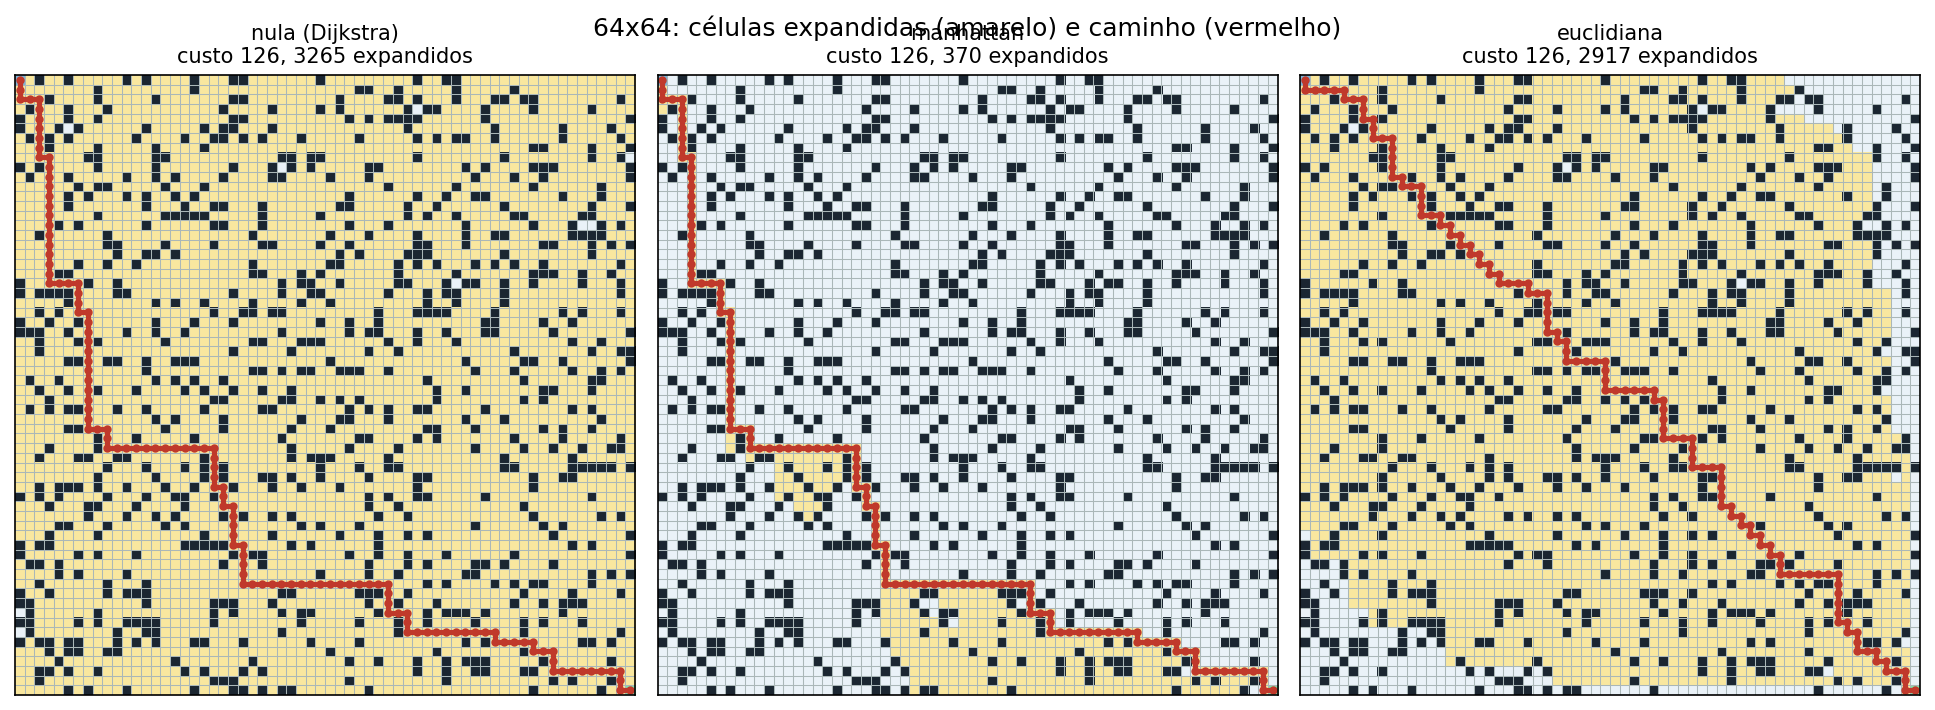
\includegraphics[width=\linewidth]{cenario_64x64.png}
  \caption{Mesmo mapa 64x64 com as três heurísticas admissíveis. O caminho tem o mesmo custo, mas a Manhattan expande
    uma faixa estreita em volta dele, enquanto Dijkstra e Euclidiana varrem quase o mapa todo.}
  \label{fig:64}
\end{figure}

\subsubsection*{Posições do início e do objetivo}

\begin{table}[H]
  \centering
  \small
  \caption{Mesmo mapa 16x16 com S e G em lugares diferentes.}
  \label{tab:posicoes}
  \begin{tabular}{lccrrrr}
    \toprule
    posições & S & G & $h(S)$ & custo & Dijkstra & Manhattan \\
    \midrule
    cantos opostos         & (0,0)   & (15,15) & 30 & 30 & 202 & 45 \\
    mesmo lado             & (0,0)   & (0,15)  & 15 & 17 &  96 & 17 \\
    centro $\to$ canto     & (8,8)   & (15,15) & 14 & 14 & 193 & 23 \\
    canto $\to$ centro     & (15,15) & (8,8)   & 14 & 14 &  67 & 14 \\
    vizinhos na diagonal   & (7,7)   & (8,8)   &  2 &  2 &   9 &  2 \\
    objetivo entre buracos & (0,0)   & (2,5)   &  7 &  7 &  25 & 12 \\
    \bottomrule
  \end{tabular}
\end{table}

\subsubsection*{Densidade de buracos}

\begin{table}[H]
  \centering
  \small
  \caption{50 mapas 32x32 por valor de $p$, sem filtrar os mapas sem caminho. A Manhattan inicial é sempre 62.
    As colunas de custo e de nós expandidos usam só os mapas com caminho.}
  \label{tab:densidade}
  \begin{tabular}{rrrrrrr}
    \toprule
    $p$ & \% com caminho & custo médio & custo / $h(S)$ & Dijkstra & Manhattan & economia (\%) \\
    \midrule
    1,00 & 100 & 62,00 & 1,00 & 1023,0 &  62,0 & 93,9 \\
    0,90 & 100 & 62,00 & 1,00 &  919,2 & 103,1 & 88,8 \\
    0,80 &  86 & 62,05 & 1,00 &  814,4 & 131,7 & 83,8 \\
    0,70 &  40 & 63,10 & 1,02 &  691,7 & 181,2 & 73,8 \\
    0,65 &  26 & 66,31 & 1,07 &  587,4 & 234,8 & 60,0 \\
    0,60 &   8 & 80,00 & 1,29 &  412,3 & 267,5 & 35,1 \\
    \bottomrule
  \end{tabular}
\end{table}

\begin{figure}[H]
  \centering
  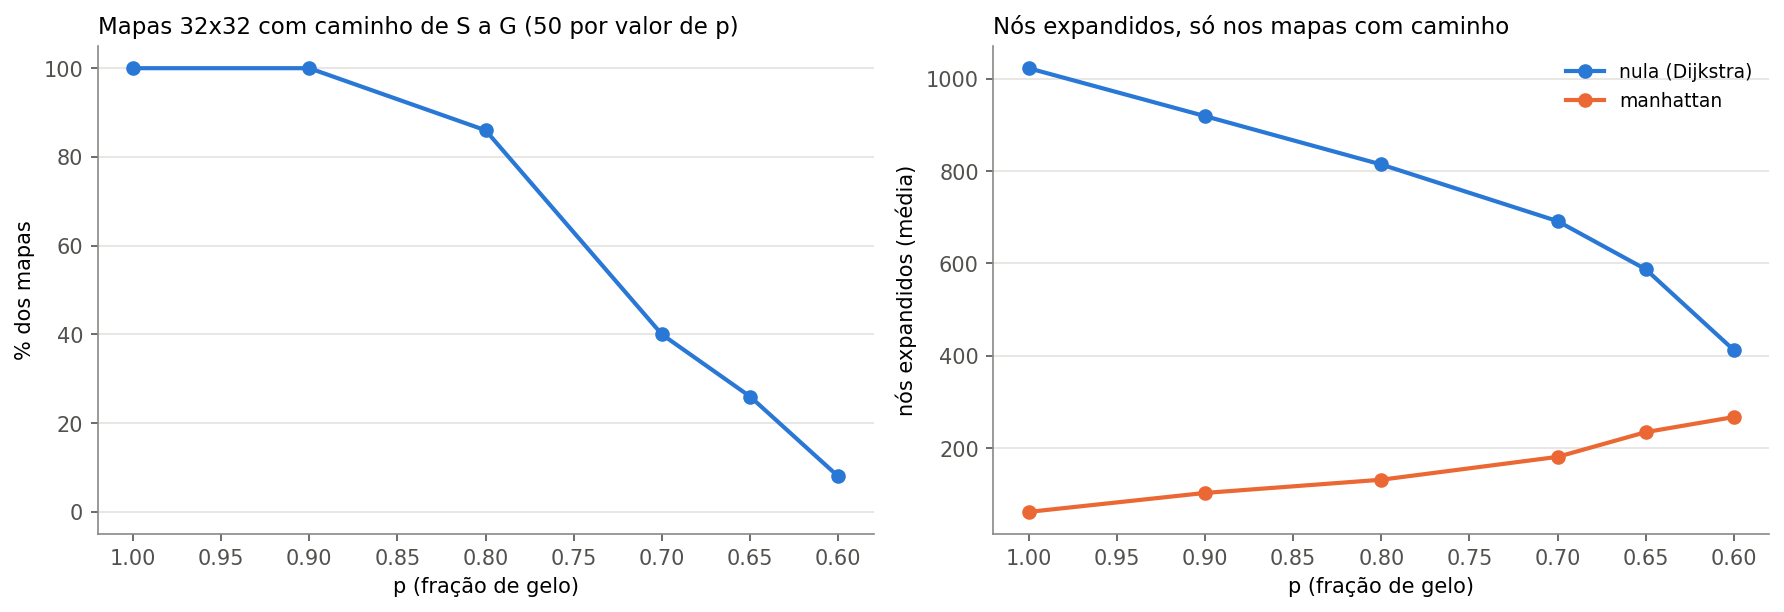
\includegraphics[width=\linewidth]{cenario_densidade.png}
  \caption{À esquerda, a fração de mapas com caminho cai de forma brusca entre $p = 0{,}8$ e $p = 0{,}6$. À direita, os
    nós expandidos nos mapas com caminho.}
  \label{fig:densidade}
\end{figure}

\subsubsection*{Padrões montados à mão e mapas sem solução}

\begin{table}[H]
  \centering
  \small
  \caption{Padrões que isolam casos em que a Manhattan é enganada (nós expandidos).}
  \label{tab:padroes}
  \begin{tabular}{lrrrrrr}
    \toprule
    padrão & $h(S)$ & custo & alcançáveis & Dijkstra & Manhattan & Euclidiana \\
    \midrule
    parede, passagem alinhada & 15 &  15 & 241 & 170 &  15 &  15 \\
    parede, passagem na ponta & 15 &  31 & 241 & 212 & 136 & 178 \\
    armadilha em U            & 14 &  24 & 231 & 230 & 107 & 181 \\
    labirinto perfeito        & 60 & 264 & 511 & 346 & 315 & 316 \\
    labirinto com ciclos      & 60 &  84 & 533 & 514 & 341 & 434 \\
    \bottomrule
  \end{tabular}
\end{table}

\begin{figure}[H]
  \centering
  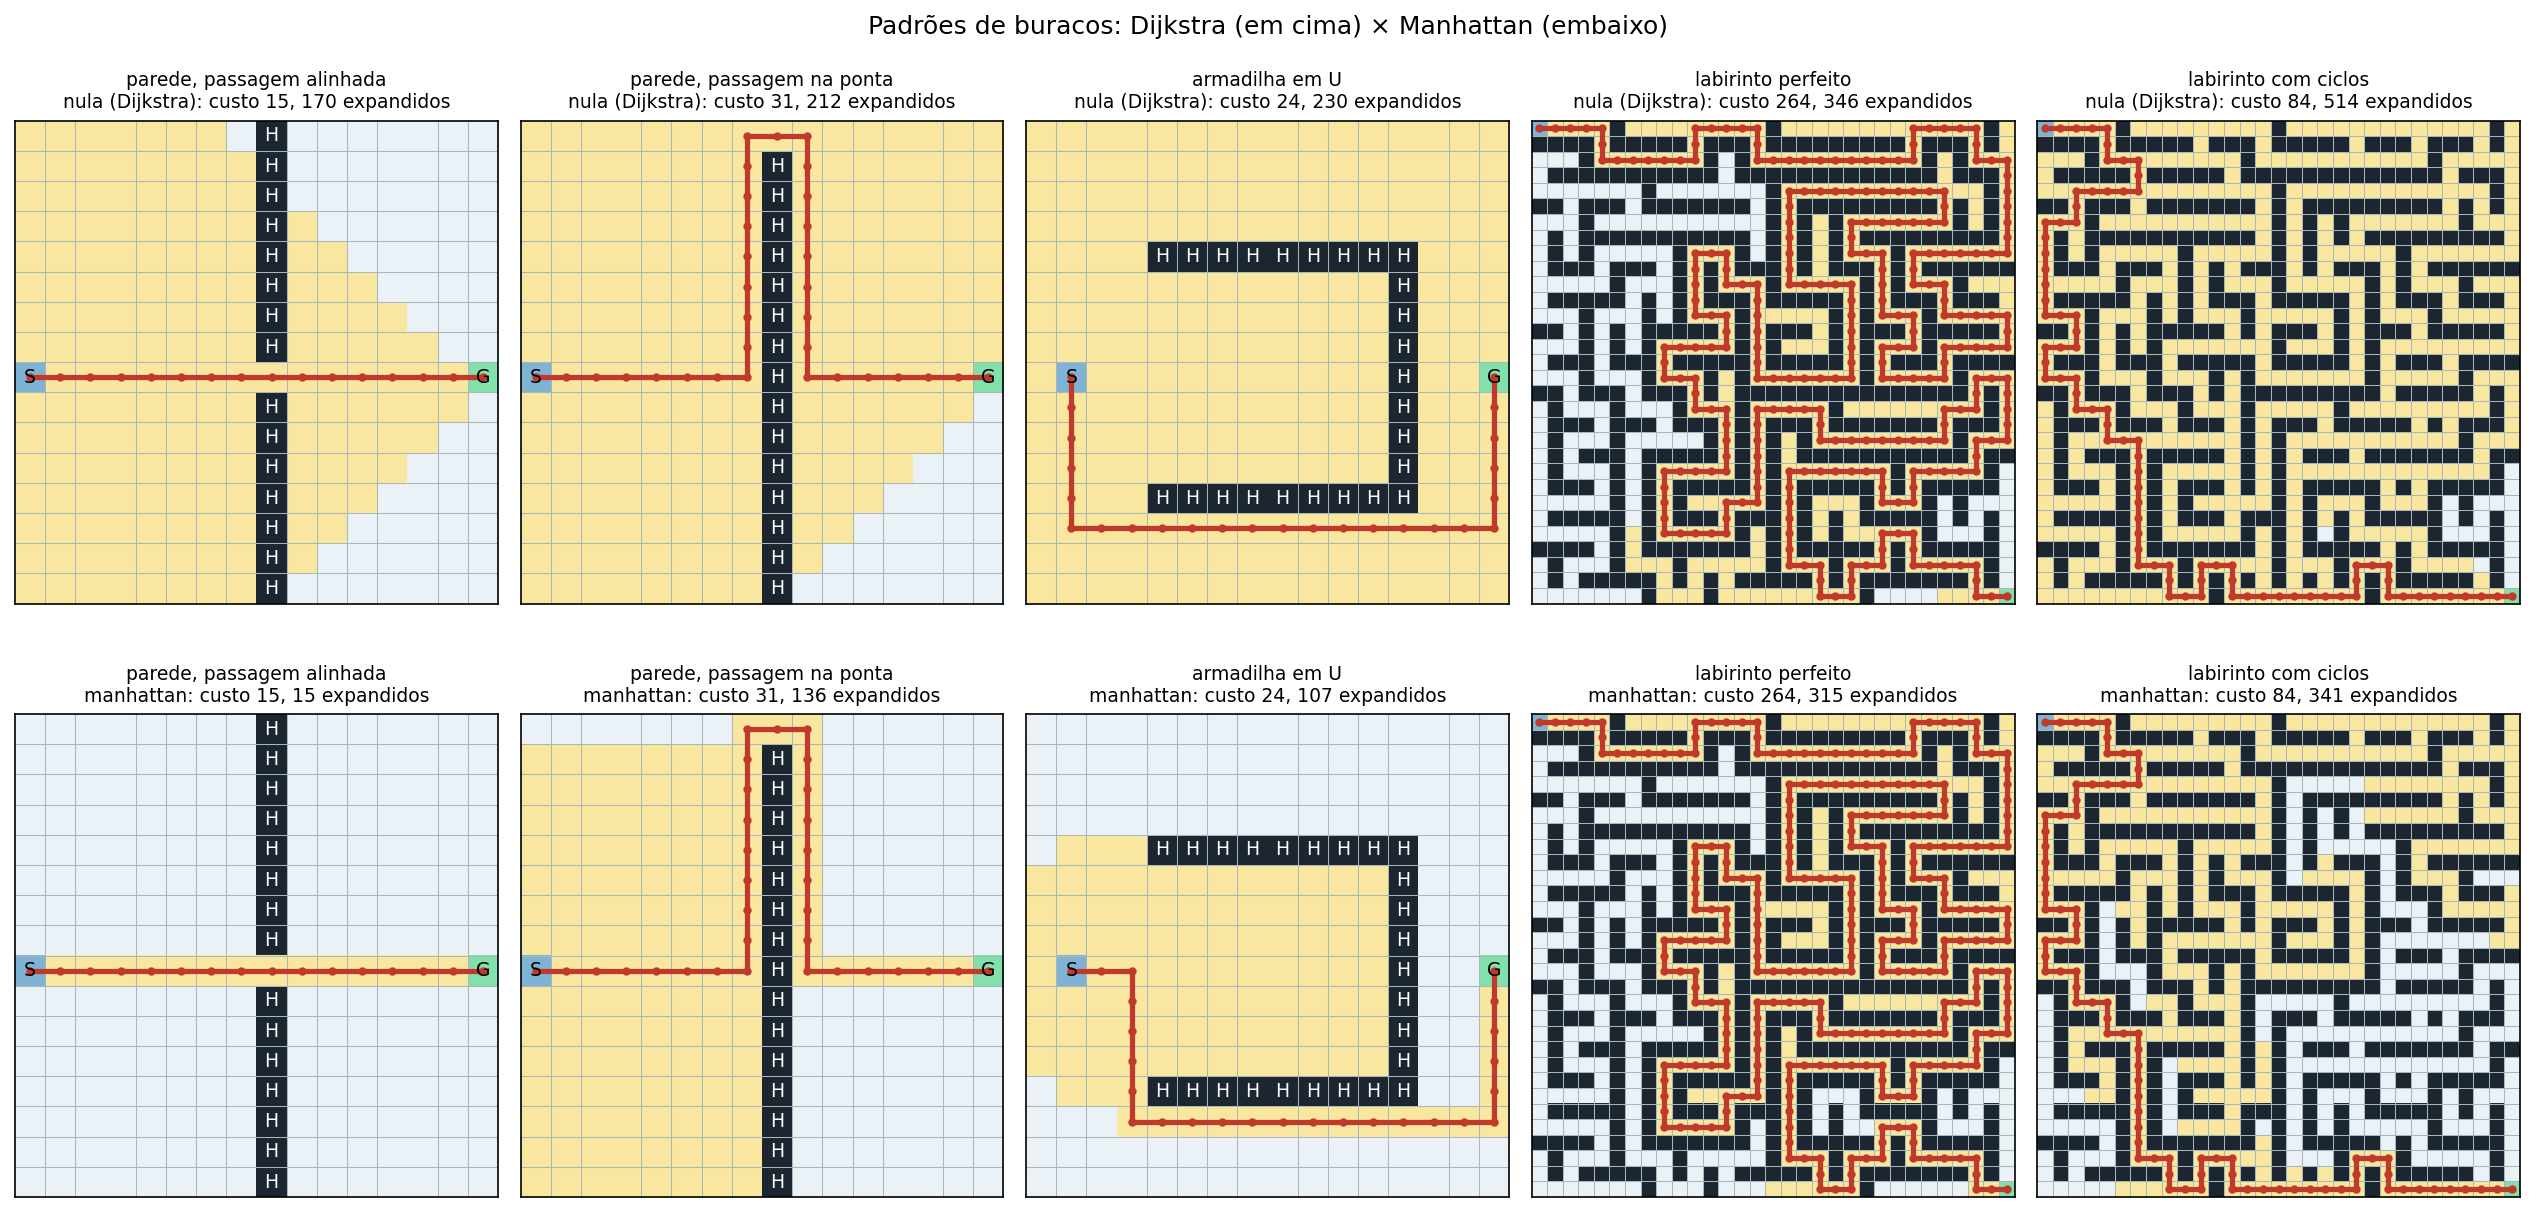
\includegraphics[width=\linewidth]{cenario_padroes.png}
  \caption{Padrões de buracos com Dijkstra (em cima) e Manhattan (embaixo). Na armadilha em ``U'' a Manhattan puxa a
    busca para dentro do U, que fica na direção do G.}
  \label{fig:padroes}
\end{figure}

Nos mapas sem solução, toda heurística admissível expandiu exatamente as células alcançáveis a partir de S: 247 no
mapa 16x16 com o G cercado, e 29, 8 e 493 nos três mapas de $p = 0{,}6$. A Manhattan $\times 2$ expandiu 623 nós no
mapa do G cercado, mais que o número de células alcançáveis.

\subsubsection*{Heurísticas}

\begin{table}[H]
  \centering
  \small
  \caption{50 mapas 32x32 do \texttt{generate\_random\_map} com $p = 0{,}8$. Subótimo: custo acima do de Dijkstra.}
  \label{tab:heuristicas}
  \begin{tabular}{lrrrrr}
    \toprule
    heurística & expandidos & fronteira máx. & \% subótimos & excesso médio (\%) & excesso máx. (\%) \\
    \midrule
    nula (Dijkstra)  & 814,8 & 32,4 &   0 &  0,0 &  0,0 \\
    Manhattan        & 133,4 & 90,4 &   0 &  0,0 &  0,0 \\
    Euclidiana       & 695,3 & 52,4 &   0 &  0,0 &  0,0 \\
    Manhattan ×1,5   & 102,2 & 66,5 &  90 &  5,6 & 12,9 \\
    Manhattan ×2     &  97,7 & 64,4 &  98 &  9,5 & 19,4 \\
    Manhattan ×5     &  93,5 & 63,9 & 100 & 15,1 & 38,7 \\
    \bottomrule
  \end{tabular}
\end{table}

Com $p = 0{,}7$ o comportamento se repete: a Manhattan $\times 1{,}5$ fica subótima em 74\% dos mapas, e o excesso
máximo chega a 53,1\% com $w = 5$. Nos padrões, só o labirinto com ciclos foi afetado (custo 84 $\to$ 96 com $w = 2$
e 108 com $w = 5$).

\begin{figure}[H]
  \centering
  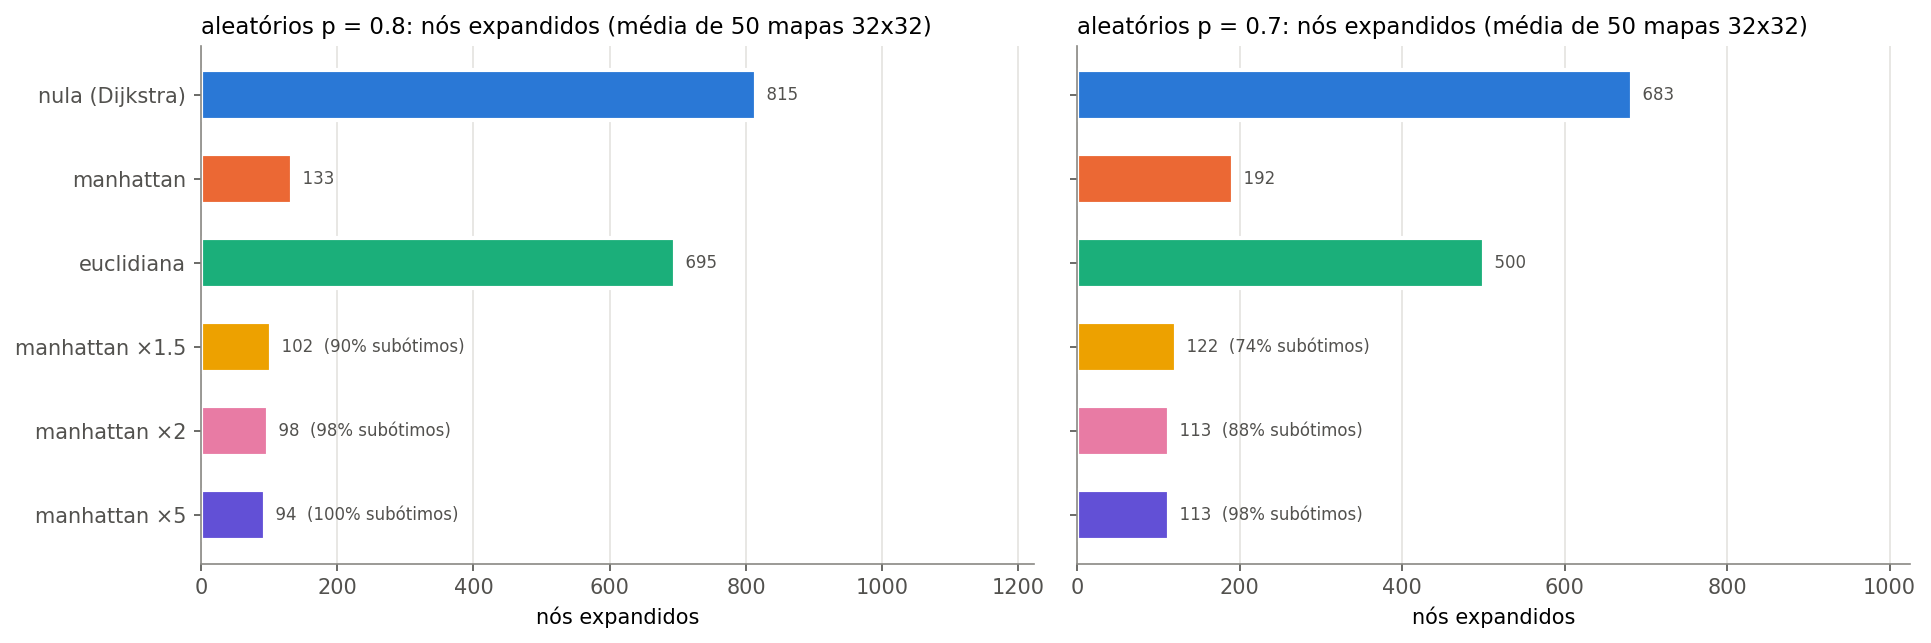
\includegraphics[width=\linewidth]{cenario_heuristicas.png}
  \caption{Nós expandidos por heurística nos mapas aleatórios 32x32. Entre parênteses, a fração de mapas em que o
    caminho saiu mais caro que o ótimo.}
  \label{fig:heuristicas}
\end{figure}

\subsection{Eixo 2: custo inspirado no Uber}

\subsubsection*{Camadas do grid}

\begin{figure}[H]
  \centering
  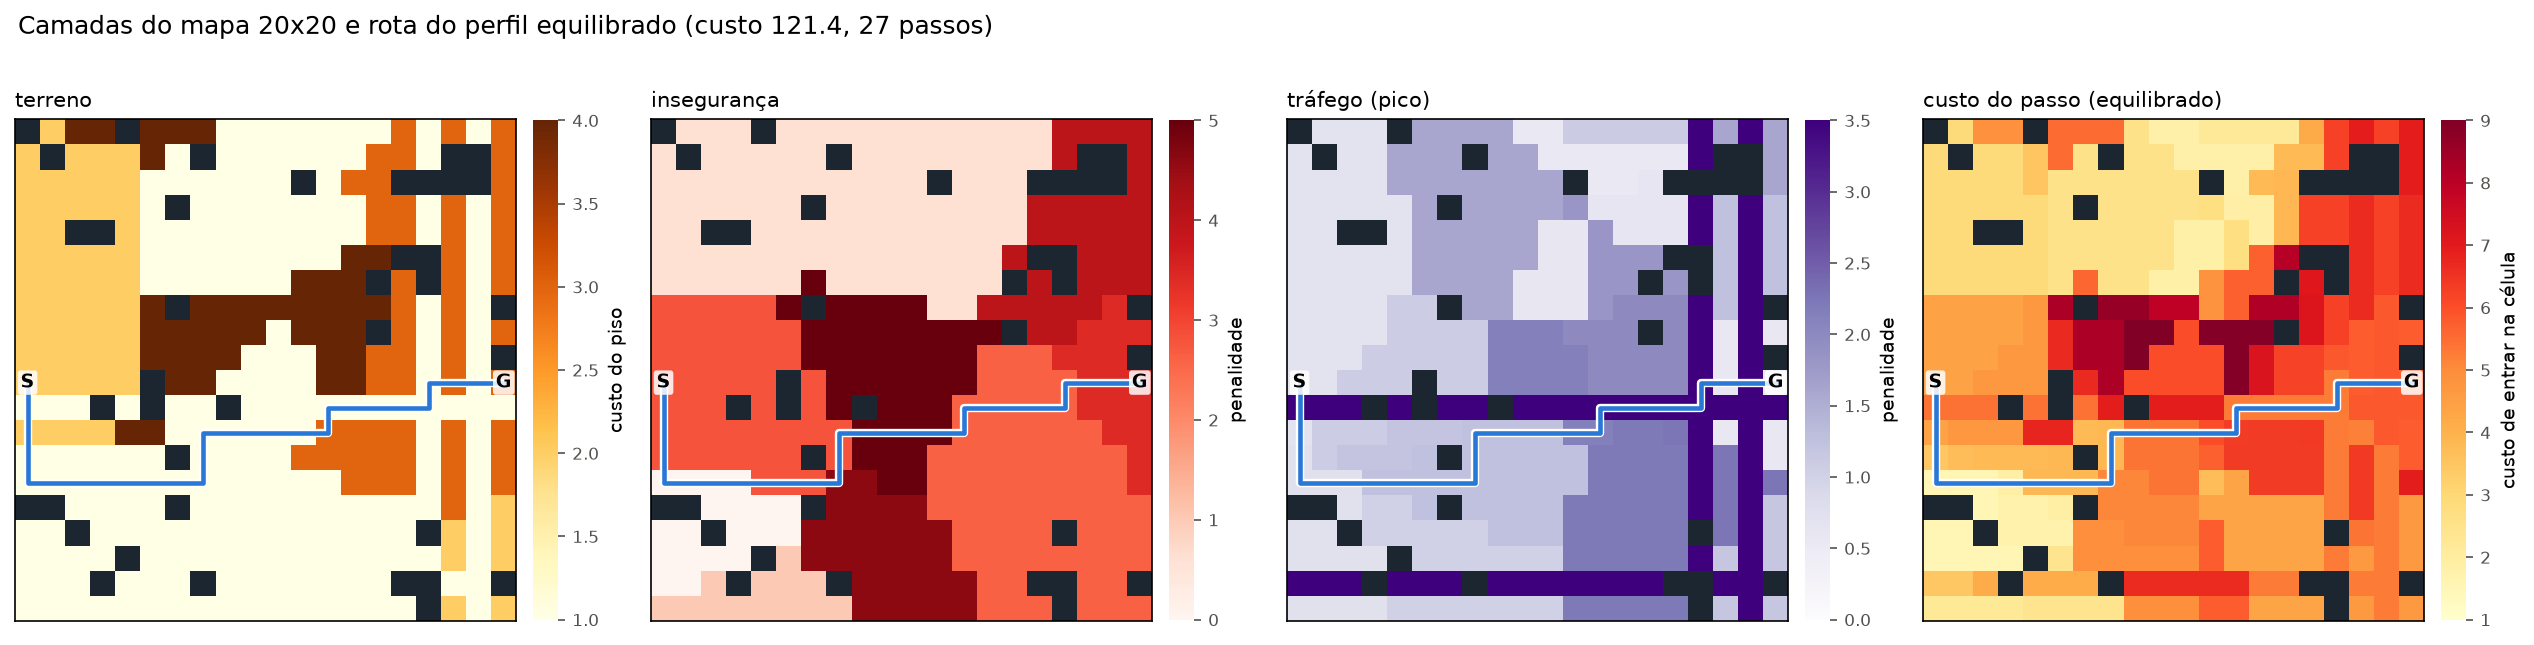
\includegraphics[width=\linewidth]{custo_camadas.png}
  \caption{Camadas do mapa de vitrine 20x20 (pico), com a rota do perfil equilibrado em azul. As camadas formam
    manchas (bairros), e não ruído célula a célula. As avenidas aparecem como faixas de asfalto no terreno e de trânsito
    máximo no tráfego. O último painel é o custo que o A* de fato enxerga. Buracos em preto.}
  \label{fig:camadas}
\end{figure}

\subsubsection*{Perfis de peso no mesmo mapa}

\begin{table}[H]
  \centering
  \small
  \caption{Mapa de vitrine, mesmos S e G e mesmas camadas (pico). Custo no próprio perfil, rota ótima de Dijkstra e
    nós expandidos. As colunas $\Sigma$ somam cada camada ao longo da rota, independentemente dos pesos.}
  \label{tab:perfis_vitrine}
  \begin{tabular}{lrrrrrrr}
    \toprule
    & & & \multicolumn{2}{c}{nós expandidos} & & & \\
    \cmidrule(lr){4-5}
    perfil & custo & passos & Dijkstra & Manh. $\times$ cmin & $\Sigma$ terreno & $\Sigma$ insegurança & $\Sigma$ tráfego \\
    \midrule
    mais rápido &  82,4 & 25 & 359 & 343 & 33,0 & 82,4 & 49,4 \\
    mais seguro & 151,8 & 29 & 346 & 337 & 62,0 & 50,2 & 41,6 \\
    equilibrado & 121,4 & 27 & 360 & 360 & 34,0 & 75,4 & 49,4 \\
    \bottomrule
  \end{tabular}
\end{table}

\begin{table}[H]
  \centering
  \small
  \caption{Cada rota (linhas) avaliada com a função de custo de cada perfil (colunas). O menor valor de cada coluna
    está na diagonal: cada rota é a melhor só para o próprio perfil.}
  \label{tab:cruzada}
  \begin{tabular}{lrrr}
    \toprule
    & \multicolumn{3}{c}{custo no perfil} \\
    \cmidrule(lr){2-4}
    rota & mais rápido & mais seguro & equilibrado \\
    \midrule
    mais rápido & \textbf{82,4} & 207,0 & 125,3 \\
    mais seguro & 103,6 & \textbf{151,8} & 126,2 \\
    equilibrado & 83,4 & 194,7 & \textbf{121,4} \\
    \bottomrule
  \end{tabular}
\end{table}

\begin{figure}[H]
  \centering
  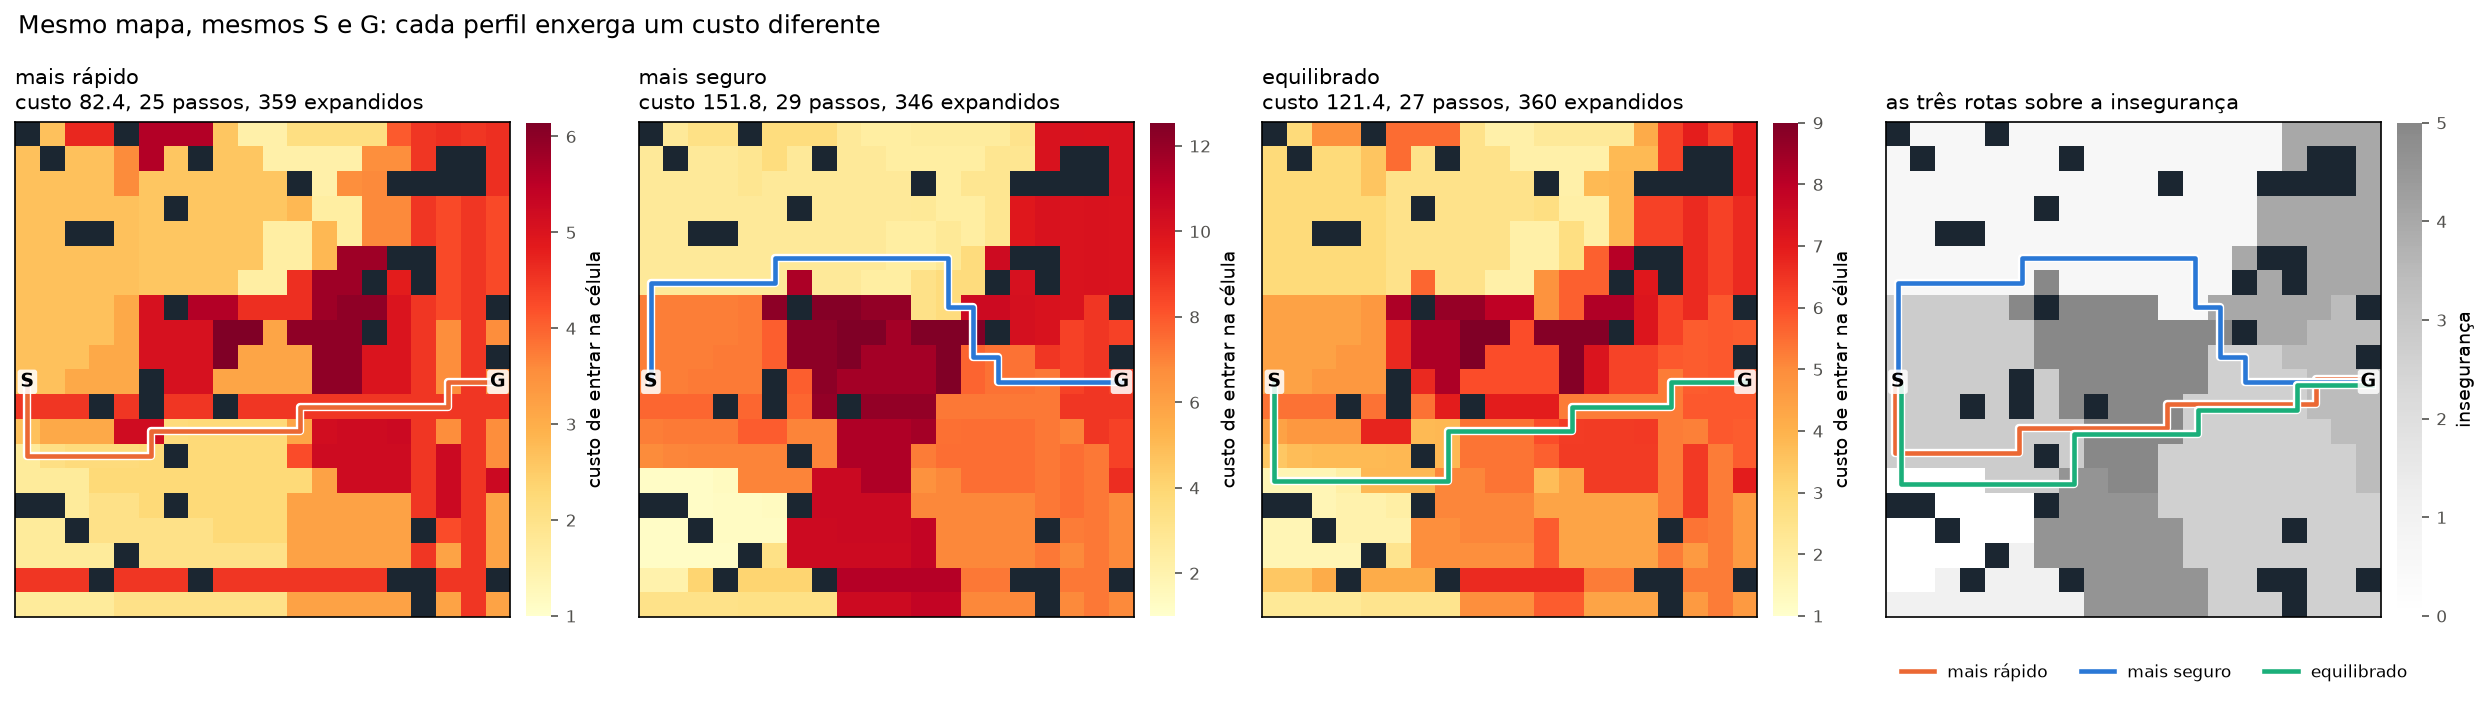
\includegraphics[width=\linewidth]{custo_perfis.png}
  \caption{As rotas dos três perfis no mapa de vitrine, cada uma sobre o custo que o seu perfil enxerga. No último
    painel, as três rotas sobre a camada de insegurança: a mais segura dá a volta por cima do bairro perigoso.}
  \label{fig:perfis}
\end{figure}

\subsubsection*{Perfis em vários mapas}

\begin{table}[H]
  \centering
  \small
  \caption{Quantas rotas diferentes os três perfis produzem no mesmo mapa (15 mapas por linha, pico).}
  \label{tab:divergencia}
  \begin{tabular}{lrrr}
    \toprule
    disposição de S e G & tamanho & \% com 3 rotas distintas & \% com pelo menos 2 \\
    \midrule
    cantos opostos & 16x16 &  73,3 & 100,0 \\
                   & 24x24 &  66,7 & 100,0 \\
                   & 32x32 & 100,0 & 100,0 \\
    mesma linha    & 16x16 &  13,3 &  53,3 \\
                   & 24x24 &  80,0 &  93,3 \\
                   & 32x32 &  80,0 & 100,0 \\
    \bottomrule
  \end{tabular}
\end{table}

\begin{table}[H]
  \centering
  \footnotesize
  \setlength{\tabcolsep}{4pt}
  \caption{Média por perfil nos 45 mapas de cada disposição (pico).}
  \label{tab:perfis_mapas}
  \begin{tabular}{llrrrrrrr}
    \toprule
    & & & & \multicolumn{2}{c}{nós expandidos} & & & \\
    \cmidrule(lr){5-6}
    disposição & perfil & custo & passos & Dijkstra & Manh. $\times$ cmin & $\Sigma$ terreno & $\Sigma$ inseg. & $\Sigma$ tráfego \\
    \midrule
    cantos opostos & mais rápido & 129,9 & 46,1 & 554,7 & 528,5 & 62,9 & 85,1 & 67,0 \\
                   & mais seguro & 177,0 & 46,3 & 539,0 & 485,4 & 73,2 & 49,9 & 76,0 \\
                   & equilibrado & 154,8 & 46,1 & 553,8 & 516,3 & 63,8 & 56,7 & 73,3 \\
    mesma linha    & mais rápido &  82,9 & 27,2 & 480,9 & 273,4 & 41,4 & 49,5 & 41,6 \\
                   & mais seguro & 122,1 & 29,9 & 476,7 & 358,7 & 50,4 & 35,8 & 48,4 \\
                   & equilibrado & 101,7 & 27,4 & 481,7 & 313,0 & 41,5 & 42,3 & 43,8 \\
    \bottomrule
  \end{tabular}
\end{table}

\begin{figure}[H]
  \centering
  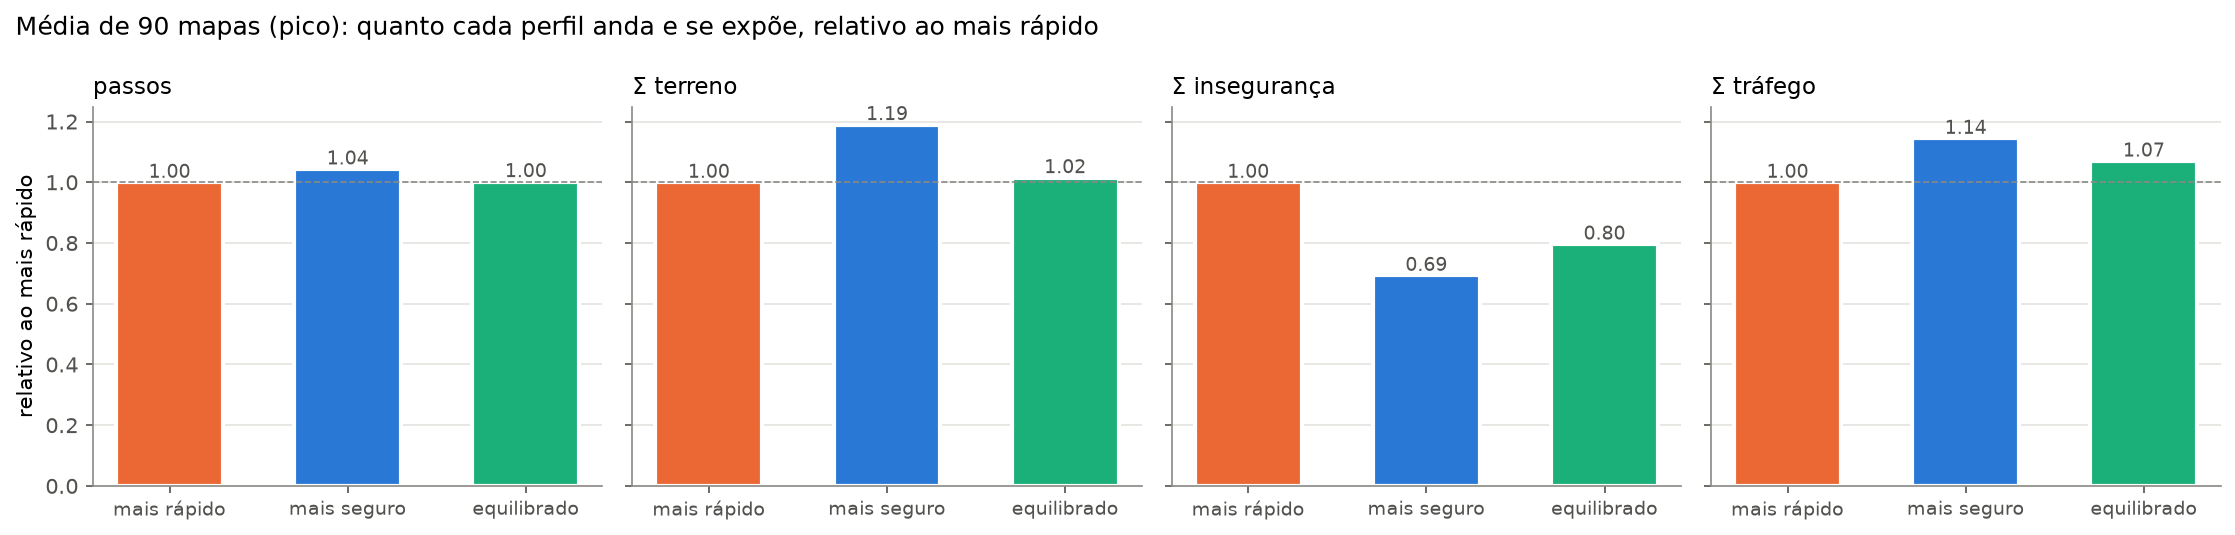
\includegraphics[width=\linewidth]{custo_perfis_mapas.png}
  \caption{Média dos 90 mapas, relativa ao perfil mais rápido do mesmo mapa. O mais seguro corta 31\% da insegurança
    acumulada com 4\% de passos a mais; o equilibrado corta 20\% sem andar mais.}
  \label{fig:perfis_mapas}
\end{figure}

\subsubsection*{Heurísticas e admissibilidade com custo variável}

A Manhattan $\times$ cmin é admissível porque qualquer caminho até o G tem pelo menos Manhattan passos, e cada um custa
pelo menos cmin. Com o custo médio ou máximo, a estimativa pode passar do custo real.

\begin{table}[H]
  \centering
  \small
  \caption{90 mapas por perfil (pico). Subótimo: custo acima do de Dijkstra. O cmin médio é 1,60 (mais rápido),
    1,72 (mais seguro) e 1,74 (equilibrado); o custo médio de passo é 3,54, 5,54 e 4,33.}
  \label{tab:heuristicas_custo}
  \begin{tabular}{lrrrrrrr}
    \toprule
    & \multicolumn{3}{c}{nós expandidos} & \multicolumn{3}{c}{\% subótimos} & excesso \\
    \cmidrule(lr){2-4}\cmidrule(lr){5-7}
    heurística & rápido & seguro & equil. & rápido & seguro & equil. & máx. (\%) \\
    \midrule
    nula (Dijkstra)                 & 517,8 & 507,8 & 517,7 &    0 &    0 &    0 &    0 \\
    Manhattan                       & 461,7 & 462,0 & 472,2 &    0 &    0 &    0 &    0 \\
    Manhattan $\times$ cmin         & 400,9 & 422,1 & 414,7 &    0 &    0 &    0 &    0 \\
    Manhattan $\times$ média        &  83,0 & 109,5 &  76,5 & 74,4 & 77,8 & 75,6 & 35,7 \\
    Manhattan $\times$ máx.         &  40,5 &  40,2 &  39,9 & 91,1 & 93,3 & 93,3 & 87,4 \\
    $2 \times$ Manhattan $\times$ cmin & 137,8 & 309,8 & 201,7 & 63,3 & 25,6 & 38,9 & 20,2 \\
    \bottomrule
  \end{tabular}
\end{table}

\begin{figure}[H]
  \centering
  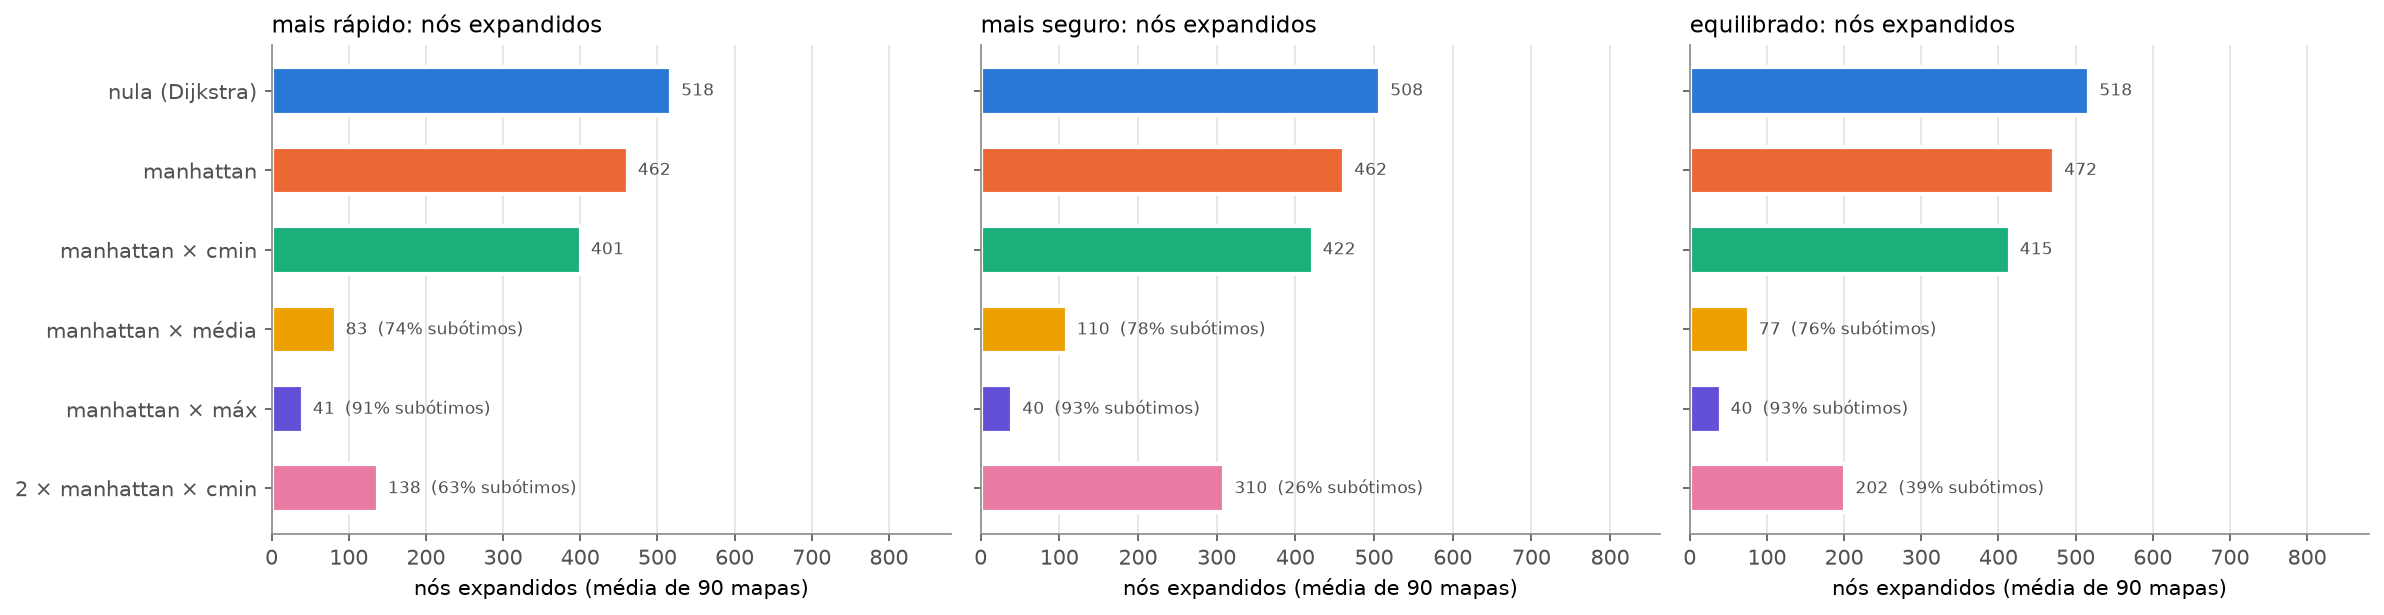
\includegraphics[width=\linewidth]{custo_heuristicas.png}
  \caption{Nós expandidos por heurística e perfil (média de 90 mapas). Entre parênteses, a fração de mapas com
    caminho mais caro que o ótimo.}
  \label{fig:heuristicas_custo}
\end{figure}

\begin{figure}[H]
  \centering
  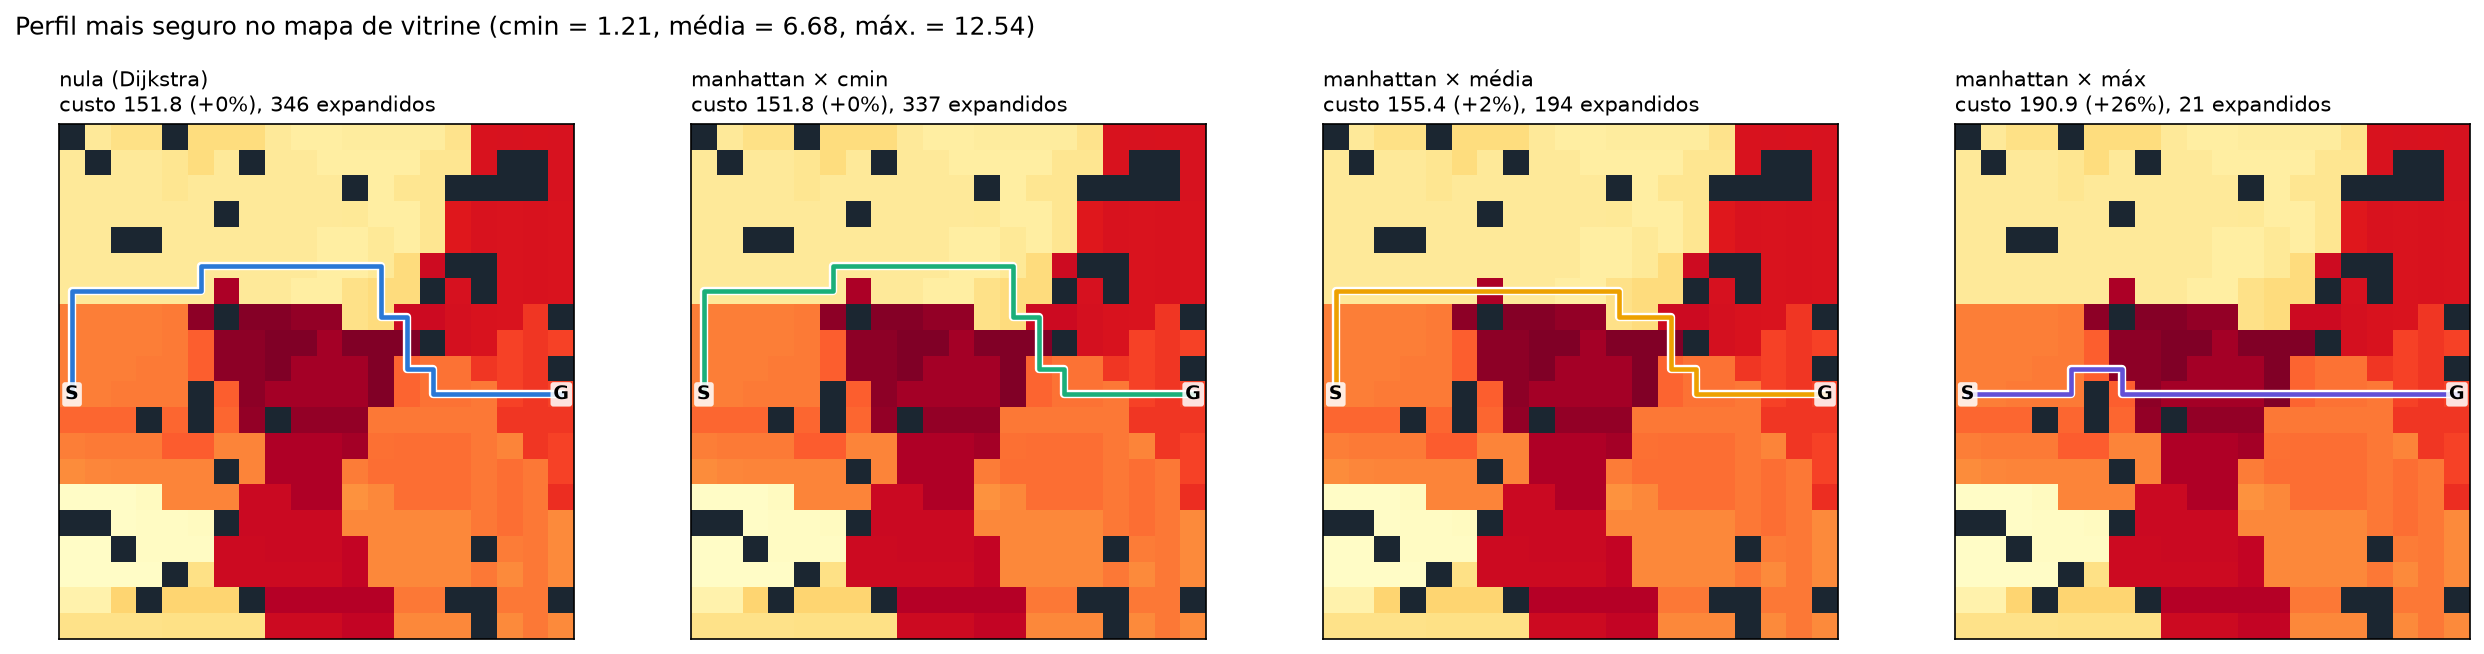
\includegraphics[width=\linewidth]{custo_admissibilidade.png}
  \caption{Perfil mais seguro no mapa de vitrine. As duas heurísticas admissíveis acham a rota ótima (151,8). A
    Manhattan $\times$ média paga 2\% a mais, e a Manhattan $\times$ máx. atravessa o bairro perigoso em linha reta,
    expande só 21 nós e paga 26\% a mais.}
  \label{fig:admissibilidade}
\end{figure}

\subsubsection*{Horário: pico $\times$ madrugada}

\begin{table}[H]
  \centering
  \footnotesize
  \setlength{\tabcolsep}{4pt}
  \caption{Perfil mais rápido nos 90 mapas. A cidade é a mesma; só muda a penalidade de trânsito.
    Última coluna: \% dos mapas em que a rota é igual à da madrugada.}
  \label{tab:horario}
  \begin{tabular}{lrrrrrrr}
    \toprule
    & & & & & \multicolumn{2}{c}{nós expandidos} & \\
    \cmidrule(lr){6-7}
    horário & custo & passos & \% em avenida & cmin & Manhattan & Manh. $\times$ cmin & \% iguais \\
    \midrule
    pico      & 106,4 & 36,7 &  9,0 & 1,6 & 461,7 & 400,9 &  22,2 \\
    normal    &  69,2 & 37,2 & 12,9 & 1,1 & 400,8 & 392,8 &  43,3 \\
    madrugada &  51,0 & 37,3 & 22,9 & 1,0 & 303,2 & 299,4 & 100,0 \\
    \bottomrule
  \end{tabular}
\end{table}

\begin{figure}[H]
  \centering
  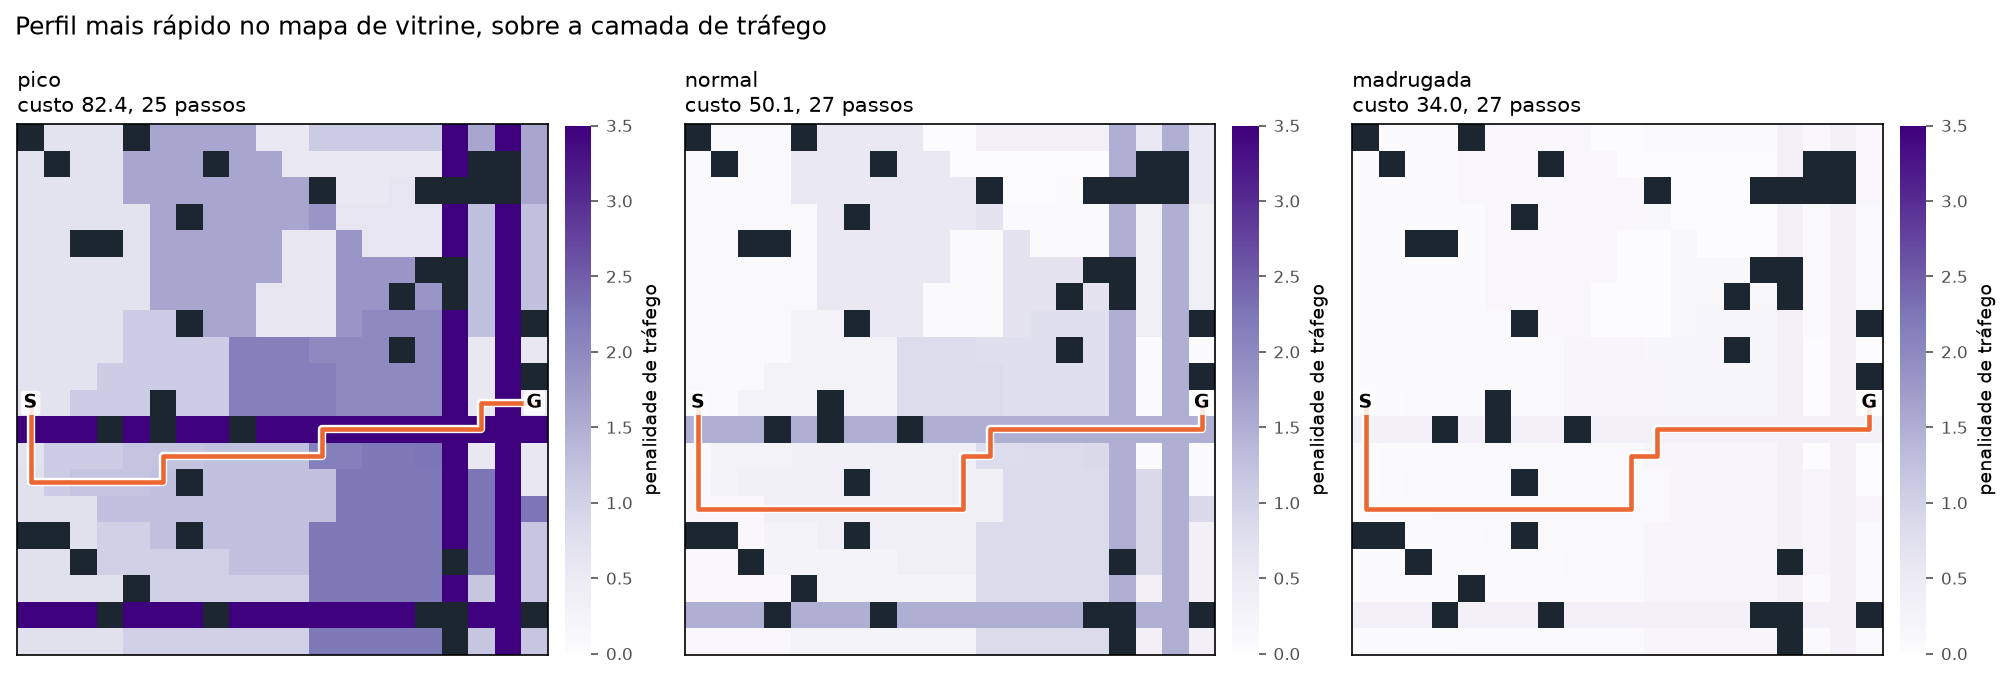
\includegraphics[width=\linewidth]{custo_horario.png}
  \caption{Perfil mais rápido no mapa de vitrine, sobre a camada de tráfego. A rota muda com o horário (25 passos no
    pico, 27 no horário normal e de madrugada).}
  \label{fig:horario}
\end{figure}

\subsubsection*{Variável extra: chuva}

\begin{table}[H]
  \centering
  \small
  \caption{90 mapas no pico, seco $\times$ chuva. Barro: células de barro na rota.}
  \label{tab:chuva}
  \begin{tabular}{lrrrrrr}
    \toprule
    perfil & custo seco & custo chuva & aumento (\%) & barro seco & barro chuva & \% rotas que mudam \\
    \midrule
    mais rápido & 106,4 & 143,7 & 35,0 & 2,9 & 1,6 & 45,6 \\
    mais seguro & 149,6 & 163,7 &  9,4 & 4,9 & 3,6 & 50,0 \\
    equilibrado & 128,2 & 159,2 & 24,1 & 3,1 & 1,9 & 52,2 \\
    \bottomrule
  \end{tabular}
\end{table}

\begin{figure}[H]
  \centering
  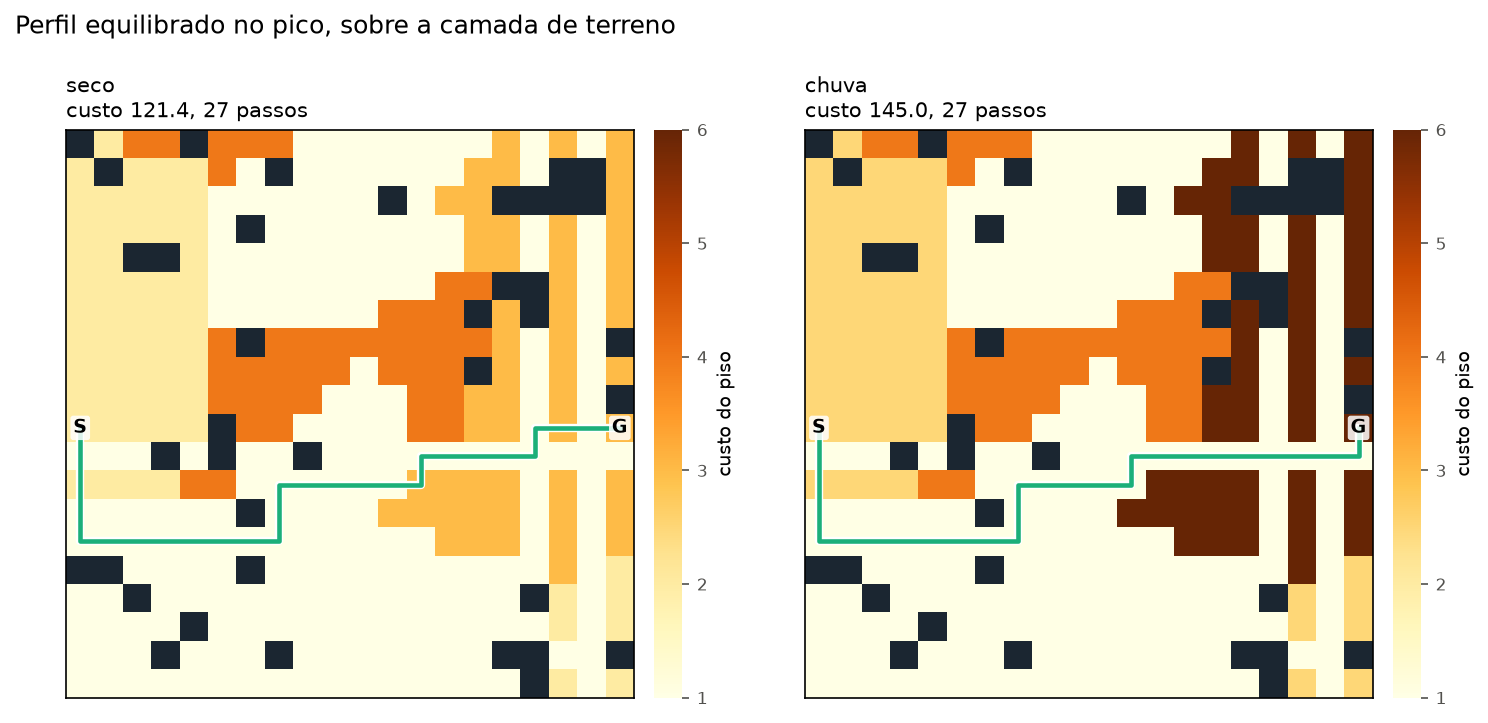
\includegraphics[width=0.8\linewidth]{custo_clima.png}
  \caption{Perfil equilibrado no mapa de vitrine, sobre a camada de terreno. Com chuva, a rota troca as células de
    barro (que passam a custar 6) por asfalto, com o mesmo número de passos.}
  \label{fig:clima}
\end{figure}

\subsection*{Análise qualitativa}

\textbf{Busca com custo 1.} Num mapa aberto, a Manhattan segue quase em linha até o objetivo. Graças ao desempate pelo
menor $h$, no mapa sem buracos ela expande exatamente os 62 nós do caminho. Quando aparece um obstáculo na direção do
objetivo, a busca ``bate'' nele e preenche a região à frente antes de contornar. Na armadilha em ``U'' (GIF no notebook)
isso fica visível: a busca enche o interior do U antes de sair pela abertura. Dijkstra, ao contrário, cresce como uma
onda uniforme em todas as direções, sem se importar com onde está o objetivo.

\textbf{Busca com custo variável.} As rotas passam a contornar bairros em vez de buracos. O perfil mais seguro troca
distância por segurança: no mapa de vitrine, anda 4 passos a mais e aceita quase o dobro de terreno ruim (33 $\to$ 62)
para reduzir a insegurança acumulada de 82 para 50. O mais rápido corta caminho pelo bairro perigoso, e o equilibrado
desvia só da parte mais crítica. No pico, as avenidas congestionadas viram uma barreira cara, e o perfil mais rápido
usa ruas paralelas; de madrugada, as avenidas voltam a ser o caminho mais barato e passam a ocupar 23\% da rota, contra
9\% no pico. Com chuva, as rotas fogem do barro quando há asfalto ao lado. A busca também muda de forma: com custos
heterogêneos, mesmo a melhor heurística admissível expande uma região larga ao redor da rota, parecida com a de
Dijkstra, em vez da faixa estreita que a Manhattan expandia com custo 1.

\section{Discussão}

\textbf{Hipóteses confirmadas.}
\begin{itemize}
  \item \textbf{H1, confirmada.} Dijkstra expande praticamente todas as células livres (de 90\% no 4x4 a 99,7\% no
    64x64), então o trabalho cresce com a área do mapa ($n^2$). Com a Manhattan, o trabalho cresce perto do comprimento
    do caminho: 366 nós para 126 passos no 64x64, ou seja, 11\% das células livres. No 64x64, o tempo cai de cerca de
    10 ms para 1,5 ms.
  \item \textbf{H2, confirmada.} A Euclidiana expande 90\% das células no 64x64, quase tanto quanto Dijkstra. De (0,0)
    a (31,31) ela estima 43,8 para um custo de 62. Ser admissível garante o caminho ótimo, mas não diz nada sobre
    eficiência. Para isso, a heurística precisa ficar perto do custo real.
  \item \textbf{H3, confirmada.} Com mais buracos, a economia da Manhattan cai de 94\% ($p = 1$) para 35\% ($p = 0{,}6$).
    Nos padrões, ela é exata com a passagem alinhada (15 nós), mas com a passagem na ponta a estimativa é metade do custo
    e a busca varre a metade esquerda do mapa (136 nós). No labirinto perfeito ela quase não ajuda (315 contra 346).
  \item \textbf{H4, confirmada.} A Manhattan $\times 1{,}5$ expande 23\% menos nós que a Manhattan, mas em 90\% dos mapas
    devolveu um caminho mais caro. Aumentar o peso quase não economiza mais nós depois de $w = 1{,}5$ e só piora o
    caminho.
  \item \textbf{H5, confirmada.} No mapa de vitrine, os três perfis fazem três rotas diferentes (25, 29 e 27 passos), e
    cada uma é a mais barata só no próprio perfil (Tabela~\ref{tab:cruzada}). Nos 90 mapas, pelo menos dois perfis
    divergem em 100\% dos mapas com S e G em cantos opostos. A exceção é o 16x16 com S e G na mesma linha, em que os
    três só divergem em 13\% dos mapas: o mapa é pequeno e desviar custa passos demais.
  \item \textbf{H6, confirmada.} Com Manhattan e Manhattan $\times$ cmin, o custo foi igual ao de Dijkstra em todas as
    540 execuções admissíveis e nas execuções de horário e chuva. A Manhattan $\times$ média ficou subótima em 74\% a
    78\% dos mapas, e a Manhattan $\times$ máx., em 91\% a 93\%, com excesso de até 87\%. A quebra não acontece em
    todos os mapas: depende de o fator passar do custo real do resto do caminho, e por isso a Manhattan $\times$ média
    ainda acerta em cerca de ¼ dos casos.
\end{itemize}

\textbf{O comportamento faz sentido com a teoria?} Sim. O A* expande todos os nós com $f(n) <$ custo ótimo, então quanto
mais $h$ subestima, mais nós entram nessa faixa. Isso explica por que a Euclidiana e a Manhattan diante de obstáculos
expandem mais. Com peso $w$, o custo encontrado ficou sempre abaixo do limite teórico do A* ponderado
($\text{custo} \le w \times \text{ótimo}$), e o pior caso foi 53\% acima do ótimo com $w = 5$, bem abaixo dos 400\%
permitidos. Nos mapas sem caminho, nenhuma heurística admissível ajuda, porque a busca só pode parar depois de provar
que o objetivo é inalcançável, e isso exige visitar toda a região conexa de S. Com a heurística que superestima foi pior
(623 expansões para 247 células), porque o A* fecha células por caminhos ruins e precisa reabri-las depois.

Dois resultados não eram esperados. Primeiro, a posição relativa importa tanto quanto a distância: ``centro $\to$
canto'' e ``canto $\to$ centro'' têm o mesmo custo, mas Dijkstra expande 193 nós num sentido e 67 no outro, porque a
partir do canto a busca só tem um quadrante para crescer. Segundo, a fração de mapas com caminho cai de 86\% para 8\%
entre $p = 0{,}8$ e $p = 0{,}6$, coerente com o limiar de percolação da grade quadrada (cerca de 59\% de células livres).
O \texttt{generate\_random\_map} do Gymnasium esconde essa transição, porque descarta os mapas sem caminho.

\textbf{Trade-off entre perfis.} Não existe ``melhor rota'' sem dizer antes o que se quer minimizar, e os pesos fazem
exatamente isso. Comparado ao mais rápido, o mais seguro reduz a insegurança acumulada em 31\%, mas anda 4\% a mais,
pega 19\% a mais de terreno ruim e 14\% a mais de trânsito. O equilibrado reduz a insegurança em 20\% com o mesmo
número de passos e quase o mesmo terreno (+2\%), então é um bom acordo. Entre as variáveis, a insegurança é a que mais
muda as rotas, porque se concentra em poucos bairros com penalidade alta. O terreno pesa menos, porque quase sempre há
asfalto por perto. O horário muda a rota do perfil mais rápido em 78\% dos mapas, e a chuva aumenta o custo em 35\%
para o perfil mais rápido, mas só 9\% para o mais seguro, que dá pouco peso ao terreno.

\textbf{Admissibilidade com custos variáveis.} Continuar admissível ficou caro. A Manhattan pura estima só 23\% a 32\%
do custo real a partir de S e economiza cerca de 10\% dos nós em relação a Dijkstra, contra 89\% no eixo de cenário.
A Manhattan $\times$ cmin é a melhor admissível testada, mas economiza só cerca de 20\%, porque o cmin (1,6 a 1,7)
fica muito abaixo do custo médio de um passo (3,5 a 5,5): a heurística precisa supor que o resto do caminho será todo
pelo bairro mais barato do mapa. Esse valor depende do horário: de madrugada o cmin cai para 1,0 no perfil mais rápido,
e aí a Manhattan $\times$ cmin vira a Manhattan pura. Do outro lado, as heurísticas que superestimam cortam de 5 a 13
vezes os nós expandidos, mas devolvem rotas piores na maioria dos mapas. A $2 \times$ Manhattan $\times$ cmin é o meio-termo
com garantia: o custo nunca passa de 2$\times$ o ótimo, e na prática o excesso máximo foi de 20\%. É a mesma troca do
A* ponderado no eixo de cenário, só que mais forte: com custos heterogêneos, a distância entre a melhor heurística
admissível e o custo real cresce, e a vantagem de superestimar aumenta.

\textbf{Limitações.}
\begin{itemize}
  \item No eixo de cenário, o custo é 1 por passo e o movimento é em 4 direções. Nesse caso a Manhattan é a melhor
    heurística possível sem obstáculos, e por isso ela parece tão boa.
  \item O ambiente é usado com \texttt{is\_slippery=False}. No lago escorregadio, a ação nem sempre leva à célula
    planejada, e o A* precisaria replanejar a cada passo ou ser trocado por uma abordagem para ambientes estocásticos,
    como o Q-learning da atividade anterior.
  \item O número de nós expandidos depende da regra de desempate (aqui, menor $h$). Com outra regra, os valores mudam,
    principalmente em mapas abertos.
  \item Os tempos são de Python e variam entre execuções; as conclusões se apoiam nos nós expandidos.
  \item As camadas de custo são sintéticas, e os pesos e as conversões (5 ocorrências = 1 ponto, base e escala do
    trânsito) foram escolhidos por nós, sem calibração com dados reais. Os resultados mostram tendências, não valores
    do mundo real.
  \item A soma ponderada escolhe um único ponto da fronteira de Pareto entre tempo, segurança e conforto. Um
    aplicativo real mostraria várias rotas e deixaria o usuário escolher.
  \item O trânsito é fixo durante a viagem. Num modelo mais realista, o custo dependeria da hora de chegada a cada
    célula, e o estado do A* teria de incluir o tempo.
  \item O custo de curva ficou de fora: a \texttt{custo\_fn(origem, destino)} não sabe de onde o agente veio, e
    modelar isso exigiria o estado (célula, direção).
  \item O Gymnasium não conhece os custos. Ele só confirma que a rota chega ao G, e a otimalidade é conferida pela
    comparação com Dijkstra.
\end{itemize}

\textbf{Melhorias possíveis.} Verificar antes se S e G estão na mesma região conexa (componentes pré-calculados), o que
evita a busca exaustiva nos mapas sem caminho. Usar heurísticas que conhecem os obstáculos, como distâncias
pré-calculadas a pontos de referência (\emph{landmarks}) ou um grafo de regiões para busca hierárquica. Permitir
movimento em 8 direções, em que a distância octil faz o papel da Manhattan. No eixo de custo, a principal melhoria
seria uma heurística admissível mais próxima do custo real, por exemplo um Dijkstra reverso a partir do G (exato,
mas caro quando o G muda) ou \emph{landmarks} calculados sobre a grade de custos, em vez de multiplicar a Manhattan por
um único fator para o mapa inteiro.

\section{Conclusões}

\begin{itemize}
  \item Uma heurística admissível garante o caminho ótimo, mas o ganho de eficiência depende de o quanto ela se
    aproxima do custo real. A Manhattan reduziu as expansões em até 89\% no 64x64; a Euclidiana, igualmente
    admissível, quase não ajudou.
  \item O formato do mapa pesa mais que o tamanho: paredes, armadilhas em ``U'' e labirintos fazem a Manhattan errar
    feio, e nesses casos o A* volta a se comportar quase como Dijkstra.
  \item Mapas sem caminho são o pior caso: a busca precisa visitar toda a região alcançável, qualquer que seja a
    heurística admissível.
  \item O A* ponderado é uma troca explícita entre velocidade e qualidade. Aqui, $w = 1{,}5$ já capturou quase todo o
    ganho de velocidade, e pesos maiores só pioraram o caminho.
  \item Com custo variável, a rota ótima depende do que se quer minimizar: no mesmo mapa, os perfis mais rápido, mais
    seguro e equilibrado escolhem rotas diferentes, e cada uma só é a melhor no próprio perfil.
  \item Custos heterogêneos enfraquecem as heurísticas admissíveis. A Manhattan $\times$ cmin garante o ótimo, mas
    economiza só cerca de 20\% dos nós; as versões que superestimam são muito mais rápidas e erram a rota na maioria
    dos mapas.
\end{itemize}

\textbf{Próximos passos.} Testar o A* no lago escorregadio com replanejamento a cada passo, comparar com o Q-learning
da atividade anterior no mesmo mapa, e experimentar heurísticas com \emph{landmarks} em mapas com muitos obstáculos.
No eixo de custo, incluir o tempo no estado para o trânsito mudar durante a viagem, modelar o custo de curva com o
estado (célula, direção) e calcular a fronteira de Pareto entre os perfis em vez de um ponto por perfil.

\end{document}
